\documentclass{article}
\usepackage{amsmath}
\usepackage{amsfonts}
\usepackage{amssymb}
\usepackage{amsthm}
\usepackage{tikz}
\usepackage{float}
\usepackage{cleveref}
\usepackage[parfill]{parskip}
\usetikzlibrary{positioning}
\usetikzlibrary{arrows}

\newtheorem{definition}{Definition}
\newcommand*{\posint}{\mathbb{Z}_+}
\newcommand*{\posreal}{\mathbb{R}_+}
\newcommand*{\uniti}{\mathbb{I}}
\newcommand*{\Prob}{\mathbb{P}}
\newcommand*{\mcs}{\mathcal{S}}
\newcommand*{\mce}{\mathcal{E}}
\newcommand*{\mcc}{\mathcal{C}}
\newcommand*{\mcr}{\mathcal{R}}
\newcommand*{\mcd}{\mathcal{D}}
\newcommand*{\clamp}[1]{\text{clamp}_{#1}}
\DeclareMathOperator{\Bern}{Bern}
\DeclareMathOperator{\Exp}{Exp}

\title{Neo-Phoebe}
\author{AzeezDa}

\begin{document}
    \maketitle

\section*{Notation and conventions}
Through this document these notational conventions will be used:
\begin{itemize}
    \item The power set of a set \(A\) is denoted by \(\mathcal{P}(A)\)
    \item The cardinality of a set \(A\) is denoted by \(|A|\)
    \item The natural numbers \(\mathbb{N}\) include 0
    \item The set of positive integers are denoted by \(\posint\)
    \item The set of positive real numbers is denoted by \(\posreal\)
    \item The unit interval \([0,1]\) is denoted by \(\uniti\)
    \item The probability measure is denoted by \(\Prob\)
    \item \(\Bern(p)\) denotes the Bernoulli distribution with parameter \(p\)
    \item \(\Exp(\lambda)\) denotes the exponential distribution with parameter \(\lambda\)
    \item For closed intervals \(S=[a,b]\), \(\clamp{S}(x) = \max(a, \min(x, b))\)
    \item The indictor function is denoted thusly \(1_S\)
\end{itemize}

\section{The Model}\label{sec:defs}
The model used to simulate is a structure that is based on a set equipped with a special partition and function.

\subsection{Compartmentation Space}
\begin{definition}[Compartmentation]\label{def:compart}
    An \(n\)-compartmentation of a set \(S\) is an ordered collection of subsets of \(S\), \((C_1, C_2, \dots C_n) \in \mathcal{P}(S)^n, n \in \posint\), such that:
    \begin{enumerate}
        \item \(C_i \cap C_j = \varnothing\), for all \(1 \leq i,j \leq n, i \neq j\)
        \item \(\bigcup_{i=1}^n C_i = S\)
    \end{enumerate}
\end{definition}

Note that Definition \ref{def:compart} is similar to a partition of a set but has a fixed size and is ordered. Therefore the definition enforces that every element of \(S\) must always be in one and only one subset in the compartmentation at a time. Also note that the compartmentation subset can written in vector/stacked form:
\[
    \begin{pmatrix}
        C_1 \\ C_2 \\ \vdots \\ C_n
    \end{pmatrix}    
\]

Now the \(n\)-compartmentation of a set is used in the following definition that makes up the whole simulation model.

\begin{definition}[Transitional Compartmentation Space]
    For a fixed \(n\), a transitional \(n\)-compartmentation space is a tuple \((S, \tau)\), such that
    \begin{itemize}
        \item \(S\) is a set
        \item \(K = \{(T, \Gamma) \mid T \subseteq S, \text{ \(\Gamma\) is a n-compartmentation of \(T\)}\}\).
        \item \(\tau : K \rightarrow K\) is a function called the transition function 
    \end{itemize}
\end{definition}

That is really it for the model. Most of the work goes to strictly defining the set Transitional Compartmentation Space of size \(n\), which will be abbreviated as TCS-\(n\).

\subsection{An Example}
This section considers an example to establish more understanding before moving on to the implementation. Let the set \(S = \mathbb{N}\). Let \((S, K, \tau)\) be a TCS-2, for a compartmentation labeled \((O, E)\). Let the transition function \(\tau\) be:
\[
\tau(k) = \begin{cases}
    (T, \begin{pmatrix}
        O\backslash\{\min(P')\} \\ E \cup \{\min(P')\}
    \end{pmatrix}) &\text{if } \min(O) \equiv 0 \mod{2} \\[1cm]
    (T, \begin{pmatrix}
        O \\ E
    \end{pmatrix})  &\text{otherwise}
\end{cases}    
\]

Consider \(T = \{0,2,4,5,6\}\) and let \(O_0 = T\) making \(E_0 = \varnothing\). Let us apply \(\tau\) on \(k_0 = (T, \begin{pmatrix}
    O_0 \\ E_0
\end{pmatrix})\) a couple of times.

\begin{enumerate}
    \item \(k_1=T(k_0) = (T, \begin{pmatrix}
        \{2,4,5,6\} \\ \{0\}
    \end{pmatrix})\)
    \item\(k_2=T(k_1) = (T, \begin{pmatrix}
        \{4,5,6\} \\ \{0,2\}
    \end{pmatrix})\)
    \item\(k_3=T(k_2) = (T, \begin{pmatrix}
        \{5,6\} \\ \{0,2,4\}
    \end{pmatrix})\)
    \item\(k_4=T(k_3) = (T, \begin{pmatrix}
        \{5,6\} \\ \{0,2,4\}
    \end{pmatrix})\)
    \item It continues to be the same value afterwards\dots
\end{enumerate}

This example is simple. But the full potential of a TCS-\(n\) shines the more we work on \(\tau\). 

\section{Implementation}
This section will explain how the definition under Section \ref{sec:defs} are implemented in the simulation.

\subsection{Definitions}
In this section we will define the parts that build up the simulation. 

\subsubsection{States and Transition Functions}\label{sec:states}
This simulation will use 5 states: \emph{Susceptible}, \emph{Exposed}, \emph{Contagious}, \emph{Recovered} and \emph{Deceased}. Their transition graph is shown in Figure \ref{fig:transgraph-1}.

\begin{figure}[H]
    \centering
    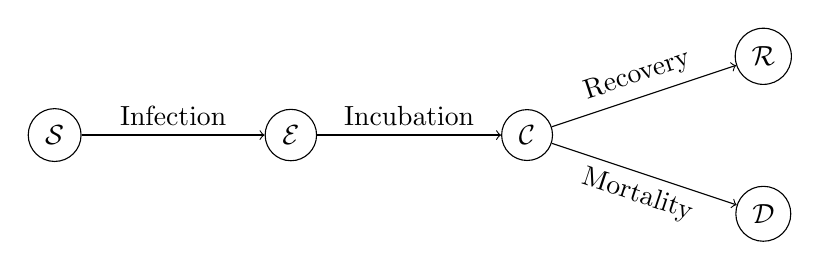
\begin{tikzpicture}[->]
        \tikzset{vertex/.style={shape=circle,draw,minimum size=1.5em}}

        \node[vertex] (S) at (0,0)  {\(\mcs\)};
        \node[vertex] (E) at (3,0)  {\(\mce\)};
        \node[vertex] (C) at (6,0)  {\(\mcc\)};
        \node[vertex] (R) at (9,1)  {\(\mcr\)};
        \node[vertex] (D) at (9,-1) {\(\mcd\)};

        \path (S) edge node[above] {Infection} (E);
        \path (E) edge node[above] {Incubation} (C);
        \path (C) edge node[above,sloped] {Recovery} (R);
        \path (C) edge node[below,sloped] {Mortality} (D);
    \end{tikzpicture}
    \caption{Graph of transitions between states}
    \label{fig:transgraph-1}
\end{figure}

\subsubsection{Population}
We define the \emph{population} to be a set \(P\) whose elements are called \emph{persons}. Additionally, we let \(\Gamma=(P, \tau)\) be a TCS-5 on \(P\) with the compartmentation labeled \((\mcs,\mce,\mcc,\mcr,\mcd)\) after the states defined in Section \ref{sec:states}.

We will say that the simulation starts with the initial 5-compartmentation of an initial subset of \(P\) denoted as \(K_0 = (\mcs_0, \mce_0, \mcc_0, \mcr_0, \mcd_0)\). Then for \(n\) applications (which we assume will be done daily) of \(\tau\) unto \(K_0\) gives \(K_n\). That is \(\tau^n(K_0) = K_n =  (\mcs_n, \mce_n, \mcc_n, \mcr_n, \mcd_n)\).

Any function \(\phi : A \rightarrow B\) that maps a subset \(A\) of the population \(P\) into any set \(B\) is called a \emph{trait}.

\subsubsection{Relationship}\label{sec:relationship}
Let \(\rho : P^2 \rightarrow \uniti\) be a function that takes two persons \(p, q \in P\) and returns the relationship strength \(\rho(p, q)\) of person \(p\) onto \(q\).

We can assume that \(\rho(p, q) = \rho(q, p)\) (which we will do during programming), but that does not affect the implementation theory.

\subsubsection{Susceptible to Exposed}
Every time unit (which we will assume to be days), a person \(p\) has a risk of being infected based on the persons \(p\) is related to. The probability of \(p\) being infected will be calculated using the relationship strength defined in Section \ref{sec:relationship}. 

First, let \(\tilde{\pi} : P^2 \rightarrow \uniti\) be a function such that for persons \(p, q \in P\), \(\tilde{\pi}(p, q)\) is the probability that person \(p\) gets infected by person \(q\). We will set \(\tilde{\pi}(p, q) = s\rho(p, q)(1-\alpha(p))(1-\alpha(q))1_{C_n}(q)\), where \(s \in \uniti\) is a constant representing the strength of disease spread, \(\alpha : P \rightarrow \uniti\) is a trait representing a persons \emph{protectiveness} or \emph{hygiencity} and \(1_C(q)\) is the indicator function that returns 1 if \(q \in C_n\) (\(q\) is contagious at day \(n\)) and 0 otherwise. (\(\tilde{\pi}\) will be slightly altered in the implementation due to disease testing and screening. See Section \ref{sec:testing} for more details).

Now a person \(p\) is considered infected if
\[
    1 = I_p = \max\{I_{p,q} \mid q \in P, I_{p, q} \in \Bern(\tilde{\pi}(p, q))\}   
\]

That is, the probability that \(p\) gets infected by any person \(q\) is Bernoulli distributed with parameter \(\tilde{\pi}(p, q)\). And \(p\) gets infected if any of those Bernoulli trials succeed.

Finding the distribution of \(I_p\) is simple if we assume that the \(I_p\)s are independent. Note that \(I_p\) is 0 if all \(I_{p,q}\) are 0. Therefore it would easier to first find \(\mathbb{P}(I_p = 0)\) then take the complement event. We do this thusly:
\begin{align*}
    \mathbb{P}(I_p = 0) &= \mathbb{P}(\max\{I_{p,q} : q \in P\} = 0) = \\
    &= \mathbb{P}\left(\bigwedge_{q \in P} I_{p,q} = 0\right) =\\
    &= \prod_{q \in P} \mathbb{P}(I_{p,q} = 0) = \\
    &= \prod_{q \in P} (1-\tilde{\pi}(p, q))
\end{align*}

Now because \(I_p\) is either 0 or 1 then \(\mathbb{P}(I_p = 1) = 1-\mathbb{P}(I_p = 0) = 1 - \prod_{q \in P} (1-\tilde{\pi}(p, q))\). This result gives that \(I_p\) is also Bernoulli distributed with the parameter \(1 - \prod_{q \in P} (1-\tilde{\pi}(p, q))\) which we will denote by \(\pi(p)\), i.e. \(I_p \in \Bern(\pi(p))\).

\subsubsection{Exposed to Contagious}\label{sec:exp-to-cont}
For every exposed person \(p \in E_n\) we define the trait \(\delta_{E_n} : E_n \rightarrow \mathbb{N}\) that counts the amount of days an since a person has been exposed:
\[
    \delta_{E_n}(p) = \sum_{i=0}^{n-1} 1_{E_i}(p)
\]
That is, it adds up 1's for every previous compartmentations where \(p\) was in \(E\) (exposed). Note that programmatically we will implement this very differently, by simply incrementing a variable.

For every exposed person \(p \in E_n\) we will assign an incubation time value given by \(X_{Cp}\), where \(X_{Cp} \in \Exp(\mu_E^{-1})\), \(\mu_E^{-1}\), where \(\mu_E \in \posreal\) is the expected (or average) incubation period for the disease.

Now we will say that a person \(p\) has transitioned from Exposed to Contagious at day \(n\) if \(\delta_{E_n}(p) \geq X_{Cp}\).

\subsubsection{Contagious to Recovered or Deceased}
Similarly to Section \ref{sec:exp-to-cont}, we define the day-counting trait \(\delta_{C_n} : C_n \rightarrow \mathbb{N}\) but now for Contagious persons thus:
\[
    \delta_{C_n}(p) = \sum_{i=0}^{n-1} 1_{C_i}(p)
\]

We also define (again similar to Section \ref{sec:exp-to-cont}) two exponential random variables that describe a person's time as Contagious before getting Recovered or Deceased. 

For every Contagious person \(p \in C_n\) we will assign \(X_{Rp}\) where \(X_{Rp} \in \Exp(\mu_R^{-1})\), \(\mu_R^{-1} \in \posreal\) corresponding to \emph{average time to get cured}.

Again, for every Contagious person we give \(X_{Dp}\) where \(X_{Dp} \in \Exp(\mu_D^{-1})\), \(\mu_D^{-1} \in \posreal\) is constant corresponding to \emph{average time before mortality}.

Now to summarise the transitions from the Contagious state at day \(n\) we define this function:
\[
\kappa_n(p)=
\begin{cases}
    1 & \text{if \(X_{Rp} \leq X_{Dp}\) and \(\delta_{C_n}(p) \geq X_{Rp}\)} \\
    -1 & \text{if \(X_{Rp} > X_{Dp}\) and \(\delta_{C_n}(p) \geq X_{Dp}\)} \\
    0 & \text{otherwise}
\end{cases}
\]
In order words, \(\kappa_n(p)\) is equal to 1 if \(p\) have recovered before deceasing, -1 if they have deceased before recovering, and 0 otherwise.

Now we say a person \(p\), at day \(n\) has transitioned from Contagious to Recovered if \(\kappa_n(p) = 1\), and from Contagious to Deceased if \(\kappa_n(p) = -1\), otherwise no transitions happened for person \(p\).

\subsection{Putting the Pieces Together}
Finally, we can define the transition \(\tau\). Assume that at day \(n\) the compartmentation of \(P\) is  \((\mcs_n, \mce_n, \mcc_n, \mcr_n, \mcd_n)\). The transition to day \(n+1\) is done thusly:
\begin{align*}
    \mcs_{n+1} &= \{p \in \mcs_n  \mid I_p = 0\} \\
    \mce_{n+1} &= \{p \in \mce_n  \mid \delta_n(p) < X_{Ep} \} \cup \{p \in \mcs_n \mid I_p = 1\} \\
    \mcc_{n+1} &= \{p \in \mcc_n  \mid \kappa_n(p) = 0\} \cup \{p \in \mce_n  \mid \delta_n(p) > X_{Ep}\} \\
    \mcr_{n+1} &= \mcr_n \cup \{p \in \mcc_n  \mid \kappa_n(p) = 1\} \\
    \mcd_{n+1} &= \mcd_n \cup \{p \in \mcc_n  \mid \kappa_n(p) = -1\}
\end{align*}

Or put in words, The Susceptible persons at day \(n+1\) are those from day \(n\) that are not infected. The Exposed persons at day \(n+1\) are persons who are still in their incubation period together with those Susceptible people at day \(n\) that have been infected. At day \(n+1\) the Contagious are those at day \(n\) that did not Recover or Decease together with those that have exceeded their incubation period. Lastly, the Recovered and Deceased at day \(n+1\) are the Recovered and Deceased from the previous day together with those that Recovered or Deceased respectively.

\subsection{Extensions: Testing, Screening and Restrictions}\label{sec:testing}
There is one last thing we will add to the model before programming it and that is a testing. It will be quite messy to model with mathematical notation so we will describe its implementation informally.

First of all we will give the simulation a non-negative integer \(t\) corresponding to the amount of tests performed per day. Now we will define three different \emph{restriction and testing plans} for the simulations.\

\subsubsection{Community Restriction}
We give the simulation a tuple \((t_\text{max}, r, d)\). Now every day we sample \(t\) persons from the population \(P\). If at least \(t_\text{max}\) persons were in \(\mce_n\) or \(\mcc_n\) then we scale \(\rho(p, q)\) by \(r\), for all \(p, q \in P\). After \(d\) days (iterations) we remove this scaling. This corresponds to responding to high positive test results by reducing people "contact" by a given factor.

For example, let \((t_\text{max}, r, d) = (5, 0.1, 60)\) and we sample \(t = 100\) per day. Then if we get for example \(13\) positively-tested persons, then we multiply \(0.1\) by all persons' relations for 60 days.

\subsubsection{Lower Cut-Off Restriction}
We give the simulation a tuple \((t_\text{max}, r, d)\). Now every day we sample \(t\) persons from the population \(P\). If at least \(t_\text{max}\) persons were in \(\mce_n\) or \(\mcc_n\) then if any \(\rho(p,q) < r\) then we set \(\rho(p,q) = 0\). After \(d\) days we remove this restriction. This restriction corresponds to responding to high positive test results by not allowing persons with low relations have any contact. This can be interpreted as only very close people are allowed to contact (such as households).

For example, let \((t_\text{max}, r, d) = (5, 0.4, 60)\) and we sample \(t = 100\) per day. Then if we get for example \(13\) positively-tested persons, then every relation between persons that is greater than \(0.4\) is set to \(0\).

\subsubsection{Upper Cut-Off Restriction}
We give the simulation a tuple \((t_\text{max}, r, d)\). Now every day we sample \(t\) persons from the population \(P\). If at least \(t_\text{max}\) persons were in \(\mce_n\) or \(\mcc_n\) then if any \(\rho(p,q) > r\) then we set \(\rho(p,q) = 0\). After \(d\) days we remove this restriction. This restriction corresponds to responding to high positive test results by not allowing persons with high probability to infect each other to meet. This can be interpreted as "protecting" highly vulnerable people to be infected by disallowing contact with people that might infect them with high probability.

\subsubsection{Personal Restriction}
We give the simulation a value \(r\). Now, every day we sample \(t\) and if any are in \(\mce_n\) or \(\mcc_n\) then we multiply their relationships with everyone else by \(r\). Note that there is no "amount of days" here since any exposed person will never be susceptible again and we need not to consider restricting or infecting them later again. This restriction corresponds to testing people daily and restricting any who turn up positive by a given factor.

For example, given \(r=0.05\), and we test \(t=100\) persons per day where \(p_2\) and \(p_5\) turned up as positive, then we multiply \(\rho(p_2, q), \rho(q, p_2), \rho(p_5, q)\) and \(\rho(q, p_5)\) by \(r\).

\subsection{Generating the Relations}
This is perhaps the most difficult thing to model in the simulation. So we will make many assumptions in order to create the relation matrix.
First of all, as previously mentioned, we will set \(\rho(p, q) = \rho(q, p)\). Next to set the values for each relation we will do two things: generate households and generate other random relations.

To generate the household relations we give the simulation a positive integer \(h\) and a relation strength value \(r \in \uniti\). Now we partition the population into sets of size \(h\) (one set might be smaller if \(h\) does not divide the population size). Then for each two persons \(p, q\) in each partition we set \(\rho(p, q) = r\).

To generate the other relations we give the simulation a list of tuples \(s,r,a\), where \(s\) and \(a\) are positive integers and \(r \in \uniti\). Now for each of this tuples we sample \(s\) persons from the population and for every two persons \(p, q\) in these samples we add \(r\) to their relation \(\rho(p, q)\) (setting it to 1 if it exceeds 1). For each tuple we do this procedure \(a\) times.

\end{document}